\chapter{Gestão de Portfólios}
\label{cap:gestao}

Esforços casuais para selecionar ações provavelmente não serão recompensados. A competição entre os investidores garante que qualquer técnica de avaliação de ações facilmente implementada será usada de maneira suficientemente ampla para que qualquer percepção extra derivada desta análise seja refletida nos preços das ações. Somente análises sérias e técnicas incomuns podem gerar o discernimento diferencial necessário para gerar lucros econômicos. Além disso, essas técnicas são economicamente viáveis apenas para gestores de grandes carteiras. Se você tem apenas R\$ 100.000 para investir, mesmo uma melhora de 1\% ao ano no desempenho gera apenas R\$ 1.000, não o suficiente para justificar grandes esforços. O gestor de um fundo de 100 milhões, no entanto, colheria um lucro extra de R\$ 1 milhão anualmente para o mesmo incremento de 1\%.

A hipótese do mercado eficiente prevê que mesmo uma análise fundamentalista acrescentará pouco valor. Se os analistas confiarem nos lucros publicamente disponíveis e nas informações do setor, a avaliação de um analista sobre as perspectivas da empresa provavelmente não será significativamente mais precisa que a de outros. Existem muitas empresas bem informadas e bem financiadas que conduzem essa pesquisa de mercado e, diante dessa concorrência, será difícil descobrir dados que também não estão disponíveis para outros analistas. Somente analistas com uma visão única seriam recompensados.

A análise fundamentalista é muito mais difícil do que simplesmente identificar empresas bem administradas e com boas perspectivas. A descoberta de boas empresas não traz lucros em excesso ao investidor se o resto do mercado também sabe que essas empresas são boas. Se o conhecimento já for público, o investidor será forçado a pagar um alto preço por essas empresas e não obterá uma taxa de retorno superior. É por isso que a análise fundamentalista é difícil. Não é suficiente fazer uma boa análise de uma empresa, você pode ganhar dinheiro (ajustado ao risco) somente se sua análise for melhor do que a de seus concorrentes, porque o preço de mercado deve refletir todas as informações normalmente disponíveis.

Os proponentes da hipótese do mercado eficiente acreditam que a administração ativa de portfólios é em grande parte um esforço desperdiçado e é improvável que justifique as despesas incorridas. Por isso, eles defendem uma estratégia de investimento passiva que não faz nenhuma tentativa de superar o mercado. Uma estratégia comum para o gerenciamento passivo é criar um fundo de índice, que é um fundo projetado para replicar o desempenho de um amplo índice de ações.

Um princípio básico na seleção de portfólio é a diversificação. Mesmo que todas as ações tenham um preço justo, cada uma delas ainda representa um risco específico da empresa, que pode ser eliminado por meio da diversificação. Portanto, a seleção racional de ativos, mesmo em um mercado eficiente, exige a seleção de um portfólio cuidadosamente diversificado. Além disso, essa carteira deve fornecer o nível de risco sistemático que o investidor deseja. Mesmo em um mercado eficiente, os investidores devem escolher os perfis de risco-retorno que considerem apropriados.

Do ponto de vista da gestão de carteiras, a questão da eficiência do mercado resume-se a se os investidores profissionais podem obter lucros econômicos anormais consistentes. O melhor teste é simplesmente olhar para o desempenho dos profissionais de mercado e ver se o seu desempenho é superior ao de um fundo de índice passivo que compra e detém uma carteira de mercado. As evidências não apoiam a afirmação de que carteiras administradas profissionalmente podem consistentemente vencer o mercado. Por outro lado, há algumas evidências fracas de persistência no desempenho, o que significa que os melhores gestores em um período tendem a continuar sendo melhores nos períodos seguintes. Tal padrão sugere que estes gestores podem, com alguma consistência, superar seus concorrentes e seria incompatível com a noção de que os preços de mercado já refletem todas as informações relevantes.

Como primeiro teste, podemos examinar os retornos ajustados ao risco (ou seja, o alfa, ou o retorno em excesso do retorno exigido com base no beta de mercado em cada período) de uma grande amostra de fundos mútuos. \citeonline{Malkiel1995}, calcula estes retornos anormais para uma grande amostra de fundos mútuos entre 1972 e 1991. Os resultados, que aparecem na figura \ref{fig:figgrosalphas}, mostram que a distribuição de alfas é aproximadamente em forma de uma normal, com uma média que é ligeiramente negativa, mas estatisticamente indistinguível de zero. 

Um artigo brasileiro de \citeonline{Castro2009} promove um estudo semelhante e compara o alfa gerado por fundos ativos e passivos no Brasil. Eles chegam a conclusão que após os custos, apenas 4,8\% dos fundos ativos possuem alfas positivos estatisticamente significativos, sendo que na média, os fundos ativos não geram retornos em excesso aos seus investidores. Refletem que seus achados estão de acordo com a formulação de eficiência de Jensen, onde os mercados são eficientes até o ponto onde os benefícios marginais de aquisição e atuação sobre informações se igualam aos custos marginais.

\begin{figure}[h]
	\centering
	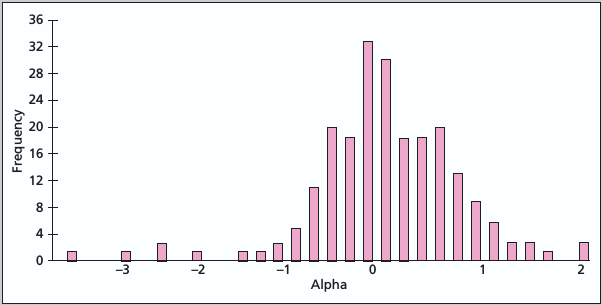
\includegraphics[width=1\linewidth]{figs/fig_gros_alphas}
	\caption[Alfas gerados por fundos americanos.]{Distribuição de alfas gerados por fundos americanos.\\ Fonte: Malkiel (1995)}
	\label{fig:figgrosalphas}
\end{figure}

Assim, as evidências sobre o desempenho ajustado ao risco dos gestores profissionais são, na melhor das hipóteses, mistas. Concluímos que o desempenho dos gestores profissionais é amplamente consistente com a eficiência do mercado. Os montantes pelos quais os gestores profissionais, enquanto grupo, batem ou não o mercado, caem na margem da incerteza estatística.

Em suma, há um papel para o gerenciamento de portfólio mesmo em um mercado eficiente. As posições ideais dos investidores variam de acordo com fatores como idade, aversão ao risco e emprego. O papel do gestor de carteira em um mercado eficiente é adequar o portfólio a essas necessidades, em vez de tentar superar o mercado.


